\documentclass[compress,xcolor=table]{beamer}
\usepackage{multicol}
\usepackage{tikz}
\usepackage{IEEEtrantools}
\usetikzlibrary{shapes}
\usetikzlibrary{arrows}
\usetikzlibrary{patterns}
\usepackage{booktabs}
\usepackage{multirow}

\usepackage{algpseudocode}

%============================================================================
% commands.tex
%============================================================================
% This file contains:
% 	- Defined Variables
%	- Redefined math shorthand
%	- Defined math shorthand


%============================================================================
% Redefined Math Commands
%============================================================================
% 	- \Vec{1} or \vec{1}
%		Long Name: Vector
%		Arguements[1]: bold and overbar arg1	
\DeclareRobustCommand{\Vec}[1]{%
    \ifmmode
        \mathbf{#1}\,%
    \else
        $\displaystyle \mathbf{#1}\,$%
    \fi
}
\DeclareRobustCommand{\vec}[1]{\Vec{#1}}

\DeclareRobustCommand{\lbm}{%
    \ifmmode
        \text{lb}_{\text{m}}
    \else
        $\displaystyle \text{lb}_{\text{m}}$%
    \fi
}
\DeclareRobustCommand{\lbf}{%
    \ifmmode
        \text{lb}_{\text{f}}
    \else
        $\displaystyle \text{lb}_{\text{f}}$
    \fi
}
\DeclareRobustCommand{\dt}{%
	\ifmmode
		\Delta t
	\else
		$\Delta t$
	\fi
}
\DeclareRobustCommand{\dtmax}{%
	\ifmmode
		\Delta t_{\text{MAX}}
	\else
		$\Delta t_{\text{MAX}}$
	\fi
}
\DeclareRobustCommand{\dx}{%
	\ifmmode
		\Delta x
	\else
		$\Delta x$
	\fi
}

\delimitershortfall-1sp
\newcommand\abs[1]{\left|#1\right|}

\DeclareRobustCommand{\BlackBox}{\State \textbf{Black Box: }}
\DeclareRobustCommand{\Test}{\State \textbf{Test: }}
\DeclareRobustCommand{\Define}{\State \textbf{Define: }}
\DeclareRobustCommand{\Update}{\State \textbf{Update: }}
\DeclareRobustCommand{\Set}{\State \textbf{Set: }}
\DeclareRobustCommand{\Calculate}{\State \textbf{Calculate: }}
%\newcommand{\algorithmicset}{\textbf{Set:}}
%\algnewcommand\Solve{\item[\algorithmicset]}

\usetheme{Szeged}
\usecolortheme{beaver}
\setbeamertemplate{navigation symbols}{}

%----------------------------------------------------------------------------
%----------------------------------------------------------------------------
\title[Department of Nuclear Engineering and Engineering Physics]{Selective Spatial-Temporal Nonlinear Refinement For
Thermal-Hydraulic Safety Analysis Codes}
\author[Lloyd]{Lewis John Lloyd}
\institute[University of Wisconsin - Madison]
{
  Department of Nuclear Engineering and Engineering Physics \\
  University of Wisconsin - Madison
}
\date[Prelim Defense 2012]{Preliminary Defense, 2012}
\subject{Nuclear Engineering}

%----------------------------------------------------------------------------
%----------------------------------------------------------------------------

\begin{document}
%------------------------------------------------------------------------------
%------------------------------------------------------------------------------

%\AtBeginSubsection[]
%{
%\begin{frame}
%\tableofcontents[subsectionstyle=show/shaded/hide,sectionstyle=show/shaded]
%\end{frame}
%}

%------------------------------------------------------------------------------
%------------------------------------------------------------------------------
\frame{\titlepage}
%------------------------------------------------
%------------------------------------------------
\begin{frame}
\begin{multicols}{2}
\tableofcontents
\end{multicols}
\end{frame}
%------------------------------------------------------------------------------
%------------------------------------------------------------------------------
\section[Background and Introduction]{Background and Introduction}
%------------------------------------------------
%------------------------------------------------
\begin{frame}
\frametitle{Introduction}

\begin{itemize}
\item{test1}
\item{test2}
\end{itemize}

\end{frame}
%------------------------------------------------------------------------------
%------------------------------------------------------------------------------
\subsection[Geometry]{Geometry of Interest}
%------------------------------------------------
%------------------------------------------------
\begin{frame}
\frametitle{Hydrodynamic Components}
\begin{columns}
\column{0.5\textwidth}

\begin{itemize}
\item{Sections}
\item{Channels}
\item{Gaps}
\end{itemize}

\column{0.5\textwidth}
\begin{figure}[t]
\centering
\resizebox{!}{0.7\textheight}{
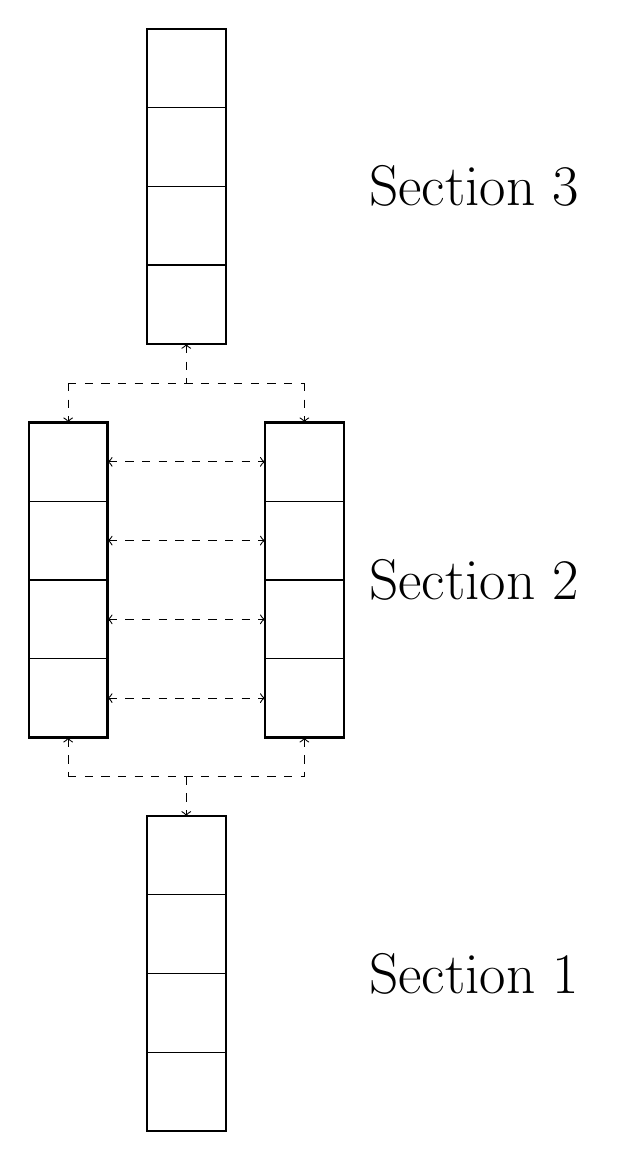
\begin{tikzpicture}
\draw [thick] (-2,-2) rectangle (-1,2);
\draw [thick] (1,-2) rectangle (2,2);
\draw [thick] (-0.5,3) rectangle (0.5,7);
\draw [thick] (-0.5,-7) rectangle (0.5,-3);
\draw [dashed] (-1.5,2.5) -- (1.5,2.5);
\draw [dashed](-1.5,-2.5) -- (1.5,-2.5);
\draw [dashed,<-] (0,3) -- (0,2.5);
\draw [dashed,->] (-1.5,2.5) -- (-1.5,2);
\draw [dashed,->] (1.5,2.5) -- (1.5,2);
\draw [dashed,->] (0,-2.5) -- (0,-3);
\draw [dashed,<-] (-1.5,-2) -- (-1.5,-2.5);
\draw [dashed,<-] (1.5,-2) -- (1.5,-2.5);
\foreach \y in {-1.5, -0.5, 0.5, 1.5}
	\draw [dashed, <->] (-1,\y) -- (1,\y);
\foreach \y in {-6,-5,-4,4,5,6}
	\draw (-0.5,\y) -- (0.5,\y);
\foreach \y in {-1,0,1}
	\draw (-2,\y) -- (-1,\y);
\foreach \y in {-1,0,1}
	\draw (1,\y) -- (2,\y);
\foreach \y/\ytext in {-5/ 1,0/ 2,5/ 3}
	\draw (2.2,\y) node [anchor=west] {\huge Section $\ytext$};
\end{tikzpicture}
}
\end{figure}

\end{columns}

\end{frame}
%------------------------------------------------
%------------------------------------------------

\begin{frame}
\frametitle{Staggered Grid}

\begin{columns}
\column{0.5\textwidth}
I will talk about staggered grids?
I may talk about staggered grids.
Who knows.
\begin{itemize}
\item{Continuity Volumes}
\item{Momentum Volumes}
\end{itemize}
\column{0.5\textwidth}
\begin{figure}
\centering
\resizebox{\textwidth}{!}{
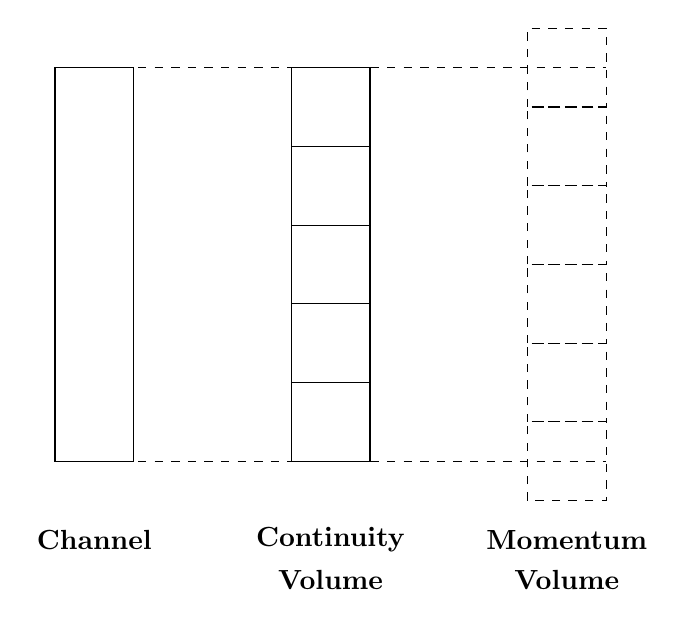
\begin{tikzpicture}
\draw (-3,0) rectangle +(1,5);
\draw (0,0) rectangle +(1,1) (0,1) rectangle +(1,1) (0, 2) rectangle +(1,1) (0,3) rectangle +(1,1) (0,4) rectangle +(1,1);
\draw[dashed] (3,-0.5) rectangle +(1,1) (3,0.5) rectangle +(1,1) (3,1.5) rectangle +(1,1) (3, 2.5) rectangle +(1,1) (3,3.5) rectangle +(1,1) (3,3.5) rectangle +(1,1) (3, 4.5) rectangle +(1,1) ;
\draw[dashed] (-3,0) -- (4,0);
\draw[dashed] (-3,5) -- (4,5);
\draw (-2.5,-1) node {\textbf{Channel}};
\draw (0.5,-1) node {\textbf{Continuity}};
\draw (0.5,-1.5) node {\textbf{Volume}};
\draw (3.5,-1) node {\textbf{Momentum}};
\draw (3.5,-1.5) node {\textbf{Volume}};
\end{tikzpicture}
}
\end{figure}
\end{columns}

\end{frame}
%------------------------------------------------------------------------------
%------------------------------------------------------------------------------
\subsection[Two-Phase Flow]{Two-Phase Flow}
%------------------------------------------------
%------------------------------------------------
\begin{frame}
\frametitle{Two-Phase Flow}

\begin{itemize}
\item{Background}
\item{Assumptions}
\item{Equations}
\end{itemize}

\end{frame}
%------------------------------------------------
%------------------------------------------------
\begin{frame}
\frametitle{Conservation of Mass}

\begin{IEEEeqnarray}{rCl}
\label{eqn:conservation_of_ncg}
\frac{\partial \left(\alpha_g \rho_{n}\right) }{\partial t } + \nabla \cdot \left( \alpha_g \rho_{n} \vec{u}_g \right) & = & s_{m,n} \nonumber \\
\label{eqn:conservation_of_vap}
\frac{\partial \left(\alpha_g \rho_v \right)}{\partial t } + \nabla \cdot \left( \alpha_g \rho_v \vec{u}_g \right)         & = & \Gamma^{'''} + s_{m,v} \nonumber \\
\label{eqn:conservation_of_liq}
\frac{\partial \left(\alpha_l \rho_l \right)}{\partial t } + \nabla \cdot \left( \alpha_l \rho_l \vec{u}_l \right)         & = & -(1-\eta)\Gamma^{'''} - S^{'''} + s_{m,l} \nonumber \\
\label{eqn:conservation_of_ent}
\frac{\partial \left(\alpha_e \rho_l \right)}{\partial t } + \nabla \cdot \left( \alpha_e \rho_l \vec{u}_e \right)         & = & -\eta\Gamma^{'''} + S^{'''}+ s_{m,e} \nonumber
\end{IEEEeqnarray}

\end{frame}
%------------------------------------------------
%------------------------------------------------
\begin{frame}
\frametitle{Conservation of Momentum}

\begin{IEEEeqnarray}{rCl}
\label{eqn:con_mom_liq}
\frac{\partial \left( \alpha_l \rho_l \vec{u}_l \right )}{\partial t } + \nabla \cdot \left( \alpha_l \rho_l \vec{u}_l \vec{u}_l \right) & = & \nonumber \\
 -\alpha_l \nabla P + \alpha_l \rho_l \vec{g} - \vec{\tau}^{'}_{w,l} + \vec{\tau}^{'}_{i,gl} - (1 - \eta)\Gamma^{'''}\vec{u}^{'} - S^{'''}\vec{u}^{'} + s_{p,l} & & \nonumber \\
\label{eqn:con_mom_gas}
\frac{\partial \left( \alpha_g \rho_g \vec{u}_g \right) }{\partial t } + \nabla \cdot \left( \alpha_g \rho_g \vec{u}_g \vec{u}_g \right) & = & \nonumber \\
 -\alpha_g \nabla P + \alpha_g \rho_g \vec{g} - \vec{\tau}^{'}_{w,g} - \vec{\tau}^{'}_{i,gl} - \vec{\tau}^{'}_{i,ge} + \Gamma^{'''}\vec{u}^{'} + s_{p,g} & & \nonumber \\
\label{eqn:con_mom_ent}
\frac{\partial \left( \alpha_e \rho_l \vec{u}_e \right) }{\partial t } + \nabla \cdot \left( \alpha_e \rho_l \vec{u}_e \vec{u}_e \right) & = & \nonumber \\
 -\alpha_e \nabla P + \alpha_e \rho_l \vec{g} - \vec{\tau}^{'}_{w,l} + \vec{\tau}^{'}_{i,ge} - \eta \Gamma^{'''}\vec{u}^{'} + S^{'''}\vec{u}^{'} + s_{p,l} & & \nonumber
\end{IEEEeqnarray}

\end{frame}
%------------------------------------------------
%------------------------------------------------
\begin{frame}
\frametitle{Conservation of Energy}

\begin{IEEEeqnarray}{rCl}
\label{eqn:con_energy_gas}
\frac{\partial \left( \alpha_g \{\rho_g h_g\} \right)}{\partial t } + \nabla \cdot \left(  \alpha_g \{\rho_g h_g\} \vec{u}_g \right) & =& \nonumber \\
\Gamma^{'''} h^{'}_v + q^{'''}_{i,v} + q^{'''}_{n,l}  + q^{'''}_{w,g} + \alpha_g\frac{\partial P}{\partial t} + s_{e,g}  & & \nonumber \\
\label{eqn:con_energy_liq}
\frac{\partial \left( (1 - \alpha_g) \rho_l h_l \right) }{\partial t } + \nabla \cdot \left( \alpha_l \rho_l h_l \vec{u}_l \right) + \nabla \cdot \left( \alpha_e \rho_l h_l \vec{u}_e \right)& = & \nonumber \\
-\Gamma^{'''} h^{'}_l +  q^{'''}_{i,l} - q^{'''}_{n,l}  + q^{'''}_{w,l} + (1 - \alpha_g) \frac{\partial P}{\partial t} + s_{e,l}  & & \nonumber
\end{IEEEeqnarray}

\end{frame}
%------------------------------------------------------------------------------
%------------------------------------------------------------------------------
\subsection[Numeric Approximation]{Numerical Approximations}
%------------------------------------------------
%------------------------------------------------
\begin{frame}
\frametitle{Spatial Approximations}

\begin{itemize}
\item{1st Order Upwind}
\item{Continuity Volume}
\item{Momentum Volume}
\end{itemize}

\end{frame}
%------------------------------------------------
%------------------------------------------------
\begin{frame}
\frametitle{Temporal Approximations}

Integrate conservation equations over a time-step.

\begin{columns}
\column{0.4\textwidth}
\begin{itemize}
\item{Single Step}
\item{Multi-Stage}
\end{itemize}
\column{0.6\textwidth}
\begin{IEEEeqnarray}{rcl}
\int^{t^{n+1}}_{t^n}\frac{\partial \vec{y}(\vec{x})}{\partial t}\mathrm{d}\tau & = & \int^{t^{n+1}}_{t^n}\vec{E}(\vec{y}(\vec{x}))\mathrm{d}\tau \nonumber \\
\vec{y}(\vec{x}^{n+1}) - \vec{y}(\vec{x}^{n}) & = & \int_{t^{n+1}}^{t^n}\vec{E}(\vec{y}(\vec{x}))\mathrm{d}\tau \nonumber  \\
\vec{y}(\vec{x}^{n+1}) - \vec{y}(\vec{x}^{n}) & = & \Delta t \vec{E}(\vec{y}(\vec{x}^{*})) \nonumber  \\
\label{eqn:simple_partial_t}
\frac{\vec{y}(\vec{x}^{n+1}) - \vec{y}(\vec{x}^{n})}{\Delta t} & = & \vec{E}(\vec{y}(\vec{x}^{*})) \nonumber
\end{IEEEeqnarray}
\end{columns}

\end{frame}
%------------------------------------------------
%------------------------------------------------
\begin{frame}
\frametitle{Nonlinear Equations}

\begin{itemize}
\item{System of nonlinear Equations.}
\item{Residuals.}
\end{itemize}

\end{frame}
%------------------------------------------------------------------------------
%------------------------------------------------------------------------------
\subsection[Solution Methods]{Solution Methods}
%------------------------------------------------
%------------------------------------------------
\begin{frame}
\frametitle{Fully-Explicit Method}

\begin{columns}
\column{0.45\textwidth}


\column{0.55\textwidth}
\begin{algorithmic}
\Require $\vec{x}^{0}$ and $t^{0}$
\Set $n = 0$
\Loop \; Take a Time Step
    \State $t^{n+1} : = t^{n} + \Delta t$
    \Calculate $\vec{F}(\vec{x}^n)$ and $\vec{J}(\vec{x}^n)$
    \Calculate $\vec{\delta x} = -\vec{J}^{-1}\vec{F}$
    \Calculate $\vec{x}^{n+1} = \vec{x}^{n} + \vec{\delta x}$ 
\EndLoop{\;$n = n+1$}
\end{algorithmic}

\end{columns}

\end{frame}
%------------------------------------------------
%------------------------------------------------
\begin{frame}
\frametitle{Fully-Implicit Method}

Here I talk about the fully-implicit method.

\end{frame}
%------------------------------------------------
%------------------------------------------------
\begin{frame}
\frametitle{Semi-Implicit Method Overview}

Semi-Implicit method.

\end{frame}
%------------------------------------------------
%------------------------------------------------
\begin{frame}
\frametitle{Semi-Implicit Method Solver}

Details

\end{frame}
%------------------------------------------------
%------------------------------------------------
\begin{frame}
\frametitle{Semi-Implicit Method Solver}

More Details

\end{frame}
%------------------------------------------------
%------------------------------------------------
\begin{frame}
\frametitle{Stability-Enhancing Two-Step Method}

Sets.

\end{frame}
%------------------------------------------------
%------------------------------------------------
\begin{frame}
\frametitle{Nearly-Implicit Method}

Nearly Implicit

\end{frame}
%------------------------------------------------------------------------------
%------------------------------------------------------------------------------
\subsection[Algorithmic Concerns]{Algorithmic Concerns}
%------------------------------------------------
%------------------------------------------------
\begin{frame}
\frametitle{Phase Transition}

Phases are transitioned.

\end{frame}
%------------------------------------------------
%------------------------------------------------
\begin{frame}
\frametitle{Time Step Failure Mitigation}

Time step failures are mitigated.

\end{frame}
%------------------------------------------------
%------------------------------------------------
\begin{frame}
\frametitle{Time-step selection}

Time step are selected.

\end{frame}
%------------------------------------------------------------------------------
%------------------------------------------------------------------------------
\subsection[Domain Coupling]{Domain Coupling}
%------------------------------------------------
%------------------------------------------------
\begin{frame}
\frametitle{Code Coupling}

Codes are coupled.

Figure of two codes talking.

\end{frame}
%------------------------------------------------
%------------------------------------------------
\begin{frame}
\frametitle{RELAP5-3D coupling}

Pressure Updates
Codes are coupled.

Figure of two codes talking.

\end{frame}
%------------------------------------------------
%------------------------------------------------
\begin{frame}
\frametitle{Domain Decomposition.}

Figure of one domain with two sub components.
Talk about additive Schwarz methods.
Talk about multiplicative Schwarz methods.

\end{frame}
%------------------------------------------------------------------------------
%------------------------------------------------------------------------------
\subsection[Research Objectives]{Research Objectives}
%------------------------------------------------
%------------------------------------------------
\begin{frame}
\frametitle{Research Objectives}

I am the objective.
Here is where I talk about stuff.
Fun stuff.

\end{frame}
%------------------------------------------------------------------------------
%------------------------------------------------------------------------------
\section[Preliminary Work]{Preliminary Work}
%------------------------------------------------
%------------------------------------------------
\subsection[COBRA]{Nonlinear COBRA}
%------------------------------------------------
%------------------------------------------------
\begin{frame}
\frametitle{Work on COBRA.}

Issues.
Coding Details
Nonlinear Solver


\end{frame}
%------------------------------------------------
%------------------------------------------------
\begin{frame}
\frametitle{Linesearch Algorithm}

Issues.
Coding Details
Nonlinear Solver


\end{frame}
%------------------------------------------------------------------------------
%------------------------------------------------------------------------------
\subsection[Scaling]{Operator Based Scaling}
%------------------------------------------------
%------------------------------------------------
\begin{frame}
\frametitle{Operator-Based Scaling}

Stuff gets scaled.

\end{frame}
%------------------------------------------------
%------------------------------------------------
\begin{frame}
\frametitle{Operator-Based Scaling}

Stuff gets scaled again.

\end{frame}
%------------------------------------------------------------------------------
%------------------------------------------------------------------------------
\subsection[Convergence]{Temporal Convergence}
%------------------------------------------------
%------------------------------------------------
\begin{frame}
\frametitle{Temporal Convergence vs Timestep Size Insensitivity}

Convergence occurs.

\end{frame}
%------------------------------------------------------------------------------
%------------------------------------------------------------------------------
\subsection[Experiments]{Numerical Experiments}
%------------------------------------------------
%------------------------------------------------
\begin{frame}
\frametitle{Numerical Experiments: Purpose}

I am the purpose.

\end{frame}
%------------------------------------------------
%------------------------------------------------
\begin{frame}
\frametitle{Numerical Experiments: Geometry}
\begin{columns}
\column{0.7\textwidth}

\begin{itemize}
\item{Cross-sectional area: 4 [in$^2$]}
\item{Total height: 48 [in]}
\item{\dx{} is constant: 4 [in]}
\item{ Boundary Conditions
	\begin{itemize}
	\item{Specified inlet flow-enthalpy}
	\item{Specified outlet pressure-enthalpy}
\end{itemize}
}
\end{itemize}

\column{0.3\textwidth}
\begin{figure}[h!t]
\centering
\resizebox{!}{0.7\textheight}{
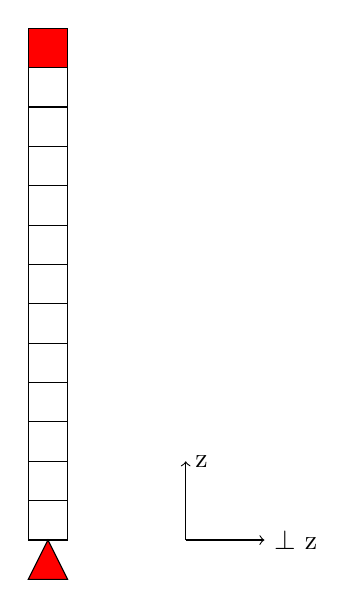
\begin{tikzpicture}
\foreach \x in {1,..., 12} \draw(0, 0.5*\x-0.5) rectangle +(.5,.5);
\filldraw[fill=red] (0, 6) rectangle +(.5,.5); 
\filldraw[fill=red] (0, -0.5) -- (0.25, 0) -- (0.5, -0.5) -- cycle;
\draw[->] (2,0) -- (2, 1) node[anchor=west] {z};
\draw[->] (2,0) -- (3, 0) node[anchor=west] {$\perp$ z};
\end{tikzpicture}
}
\end{figure}
\end{columns}
\end{frame}
%------------------------------------------------
%------------------------------------------------
\begin{frame}
\frametitle{Numerical Experiments: Initial Conditions}

\begin{table}[ht]
\centering
\begin{tabular}{@{}lr@{.}lr@{.}lr@{.}lr@{.}lr@{.}l@{}} \toprule
\multirow{2}{*}{Problem} & \multicolumn{2}{c}{Pressure} & \multicolumn{2}{c}{Enthalpy}             & \multicolumn{2}{c}{$\alpha_g$} & \multicolumn{2}{c}{$\alpha_l$} & \multicolumn{2}{c}{$\alpha_e$} \\ 
                         & \multicolumn{2}{c}{[psia]} & \multicolumn{2}{c}{$[\frac{\text{Btu}}{\lbm{}}]$} & \multicolumn{2}{c}{[-]}      & \multicolumn{2}{c}{[-]}      & \multicolumn{2}{c}{[-]}      \\ \midrule
Single-Phase             &  200&0                       &  355&5                                   & 0&0                            & 1&0                            & 0&0 \\
Flashing                 &  200&0                       & 1198&3                                   & 1&0                            & 0&0                            & 0&0 \\ \bottomrule  
\end{tabular}
\label{tab:ic}
\end{table}

\end{frame}
%------------------------------------------------
%------------------------------------------------
\begin{frame}
\frametitle{Numerical Experiments: Outlet Boundary Conditions}

\begin{table}[ht]
\centering
\begin{tabular}{@{}lr@{.}lr@{.}lr@{.}lr@{.}lr@{.}l@{}} \toprule
\multirow{2}{*}{Problem} & \multicolumn{2}{c}{Pressure} & \multicolumn{2}{c}{Enthalpy}             & \multicolumn{2}{c}{$\alpha_g$} & \multicolumn{2}{c}{$\alpha_l$} & \multicolumn{2}{c}{$\alpha_e$} \\ 
                         & \multicolumn{2}{c}{[psia]} & \multicolumn{2}{c}{$[\frac{\text{BTU}}{\lbm{}}]$} & \multicolumn{2}{c}{[-]}      & \multicolumn{2}{c}{[-]}      & \multicolumn{2}{c}{[-]}      \\ \midrule
Single-Phase             &  200&0                       &  355&5                                   & 0&0                            & 1&0                            & 0&0 \\
Flashing                 &  200&0                       & 1198&3                                   & 1&0                            & 0&0                            & 0&0 \\ \bottomrule  
\end{tabular}
\label{tab:bc_pe}
\end{table}

\end{frame}
%------------------------------------------------
%------------------------------------------------
\begin{frame}
\frametitle{Numerical Experiments: Inlet Boundary Conditions}

\begin{table}[ht]
\centering
\begin{tabular}{@{}lr@{.}lr@{.}lr@{.}lr@{.}lr@{.}l@{}} \toprule
\multirow{2}{*}{Problem} & \multicolumn{2}{c}{Pressure} & \multicolumn{2}{c}{Enthalpy}             & \multicolumn{2}{c}{$\alpha_g$} & \multicolumn{2}{c}{$\alpha_l$} & \multicolumn{2}{c}{$\alpha_e$} \\ 
                         & \multicolumn{2}{c}{[psia]} & \multicolumn{2}{c}{$[\frac{\text{BTU}}{\lbm{}}]$} & \multicolumn{2}{c}{[-]}      & \multicolumn{2}{c}{[-]}      & \multicolumn{2}{c}{[-]}      \\ \midrule
Single-Phase             &  200&0                       &  355&5                                   & 0&0                            & 1&0                            & 0&0 \\
Flashing                 & 1000&0                       &  542&6                                   & 1&0                            & 0&0                            & 0&0 \\ \bottomrule  
\end{tabular}
\label{tab:bc_fe}
\end{table}

\begin{equation*}
\label{eqn:bc_time_func_single}
\dot{m}(t) = \left\{
\begin{array}{cclrcll}
 0.0           & [\frac{ \lbm{} }{\text{s}}] & , &                & t & \leq 1 & [\text{s}] \\
 0.5 ( t - 1)  & [\frac{ \lbm{} }{\text{s}}] & , & 1\; [\text{s}] < & t & \leq 2 & [\text{s}] \\
 0.5           & [\frac{ \lbm{} }{\text{s}}] & , &                & t & > 2    & [\text{s}]
\end{array}\right.
\end{equation*}

\end{frame}
%------------------------------------------------
%------------------------------------------------
\begin{frame}
\frametitle{Numerical Experiments: Procedure}

Procedures are good.

\end{frame}
%------------------------------------------------
%------------------------------------------------
\begin{frame}
\frametitle{Numerical Experiments: Results 1}

Stuff

\end{frame}
%------------------------------------------------
%------------------------------------------------
\begin{frame}
\frametitle{Numerical Experiments: Results 2}

Results are good.

\end{frame}
%------------------------------------------------
%------------------------------------------------
\begin{frame}
\frametitle{Numerical Experiments: Results 3}

Results are better.

\end{frame}
%------------------------------------------------
%------------------------------------------------
\begin{frame}
\frametitle{Numerical Experiments: Results 4}

Results are best.

\end{frame}
%------------------------------------------------------------------------------
%------------------------------------------------------------------------------
\subsection[Review]{Review}
%------------------------------------------------
%------------------------------------------------
\begin{frame}
\frametitle{Preliminary Work Review}

Here I review.

\end{frame}
%------------------------------------------------
%------------------------------------------------
\begin{frame}
\frametitle{Preliminary Work Review}

Review part 2.

\end{frame}
%------------------------------------------------------------------------------
%------------------------------------------------------------------------------
\section[Proposed Work]{Proposed Work}
%------------------------------------------------
%------------------------------------------------
\begin{frame}
\frametitle{Proposed Timeline}


\newcommand{\cc}{\cellcolor{black}}
\begin{table}
\centering
\resizebox{0.9\textwidth}{!}{
\begin{tabular}{@{}l l c c c c  c c c c c c @{}} \toprule
Task & \multicolumn{1}{r}{Month} & Jan & Feb & Mar & Apr & May & Jun & Jul & Aug & Sep & Oct\\
\midrule
\multicolumn{12}{l}{Scaling}  \\
& Implementation & \cc & \cc &     &     &     &     &     &     &     &     \\
& Testing        &     & \cc & \cc &     &     &     &     &     &     &     \\
\multicolumn{12}{l}{Domain Decomposition} \\
& Development    & \cc & \cc &     &     &     &     &     &     &     &     \\
& Implementation &     & \cc & \cc & \cc & \cc &     &     &     &     &     \\
& Testing        &     &     &     &     & \cc & \cc &     &     &     &     \\
\multicolumn{12}{l}{Temporal Convergence Criteria}\\
& Implementation & \cc & \cc &     &     &     &     &     &     &     &     \\
& Testing        &     &     & \cc & \cc &     &     &     &     &     &     \\
\multicolumn{12}{l}{Performance Evaluation} \\
& Testing        &     &     &     &     &     & \cc & \cc &     &     &     \\
\multicolumn{12}{l}{Parametric Studies} \\
& Testing        &     &     &     &     &     & \cc & \cc & \cc &     &     \\
\multicolumn{12}{l}{Dissertation} \\
& Writing        & \cc & \cc & \cc & \cc & \cc & \cc & \cc & \cc & \cc & \cc \\
\bottomrule  
\end{tabular}
}
\end{table}

\end{frame}
%------------------------------------------------------------------------------
%------------------------------------------------------------------------------
\subsection[Scaling]{Scaling Work}
%------------------------------------------------
%------------------------------------------------
\begin{frame}
\frametitle{Proposed Scaling Work}

Scaling stuff.

\end{frame}
%------------------------------------------------------------------------------
%------------------------------------------------------------------------------
\subsection[Domain Decomposition]{Domain Decomposition}
%------------------------------------------------
%------------------------------------------------
\begin{frame}
\frametitle{Proposed Domains Decomposition}

More decomposition.

\end{frame}
%------------------------------------------------------------------------------
%------------------------------------------------------------------------------
\subsection[Testing]{Proposed Testing}
%------------------------------------------------
%------------------------------------------------
\begin{frame}
\frametitle{Proposed Testing}

Here there be testing.

\end{frame}
%------------------------------------------------------------------------------
%------------------------------------------------------------------------------
\subsection[Timeline]{Timeline}
%------------------------------------------------
%------------------------------------------------
\begin{frame}
\frametitle{Timeline}

I am stuff.

\end{frame}
%------------------------------------------------------------------------------
%------------------------------------------------------------------------------
\subsection[Possible Outcomes]{Possible Outcomes}
%------------------------------------------------
%------------------------------------------------
\begin{frame}
\frametitle{Possible Outcomes}

I am stuff.

\end{frame}
%------------------------------------------------------------------------------
%------------------------------------------------------------------------------
\section*{}
%------------------------------------------------
%------------------------------------------------
\begin{frame}
\frametitle{Acknowledgments}

This research was performed under appointment to the Rickover Fellowship Program in Nuclear Engineering sponsored by Naval Reactors Division of the U.S. Department of Energy.

\end{frame}
%------------------------------------------------
%------------------------------------------------
\begin{frame}
\frametitle{I am another extra slide.}

I am more excess.

\end{frame}
%------------------------------------------------
%------------------------------------------------
\begin{frame}
\frametitle{I am another extra slide.}

I am more excess.

\end{frame}
%------------------------------------------------------------------------------
%------------------------------------------------------------------------------
\end{document}